\documentclass[11pt]{amsart}
\usepackage{amsmath,amssymb,stmaryrd}
\setlength{\emergencystretch}{3em}
\tolerance=600
\usepackage{tikz}
\usetikzlibrary{arrows.meta,decorations.pathreplacing}
\usepackage{tikz-cd}
\usepackage[hidelinks]{hyperref}

\newtheorem{thm}{Theorem}[section]
\newtheorem{lem}[thm]{Lemma}
\newtheorem{cor}[thm]{Corollary}
\newtheorem{prop}[thm]{Proposition}
\theoremstyle{definition}
\newtheorem{defi}[thm]{Definition}
\newtheorem{rem}[thm]{Remark}
\newtheorem{ex}[thm]{Example}
\newtheorem{que}[thm]{Question}

\newcommand{\Fix}{\mathrm{Fix}}
\newcommand{\Up}{\mathrm{Up}}
\newcommand{\Nuc}{\mathrm{N}}
\newcommand{\LLJ}{\mathbf{LJ}}
\newcommand{\PLL}{\mathbf{PLL}}
\newcommand{\lax}{\bigcirc}
\newcommand{\laxa}{\bigcirc_1}
\newcommand{\laxb}{\bigcirc_2}
\newcommand{\pow}{\mathcal P}
\newcommand{\dn}{{\downarrow}}
\newcommand{\upa}{{\uparrow}}

\begin{document}

\title[Joins of relativized necessities on a poset]{Joins of relativized necessities on a poset: an alternating-chain criterion and the induction scheme of lax logic}
\author{Ryota Shibusawa}
\thanks{Corresponding author. E-mail: \texttt{r-shibusawa@daiichi-koudai.ac.jp}}
\address{Daiichi Institute of Technology}
\email{r-shibusawa@daiichi-koudai.ac.jp}
\keywords{nucleus, Heyting algebra of up-sets, relativized necessity, join of nuclei,
  lax logic, intuitionistic modal logic, frame correspondence, common knowledge}
\subjclass[2020]{03B45 (primary), 06D20, 03B20, 18F10 (secondary)}

\begin{abstract}
For a poset $P$ and a subset $C\subseteq P$, the relativized necessity
$\lax_CU=\{x:\ \upa x\cap C\subseteq U\}$ is a nucleus on the Heyting algebra
of up-sets of $P$; on a finite poset every nucleus has this form, meets of
nuclei correspond to unions of subsets and joins to intersections. We describe
the join of two relativized necessities on an arbitrary poset as a greatest
fixed point, $(\lax_C\vee\lax_{C'})(U)=P\setminus X$ with $X$ the largest
subset of $P\setminus U$ in which every point lies below a point of $X\cap C$
and below a point of $X\cap C'$, and we prove that the join equals the
necessity $\lax_{C\cap C'}$ relativized to the intersection if and only if
$P$ contains no infinite chain $q_1<q_2<\cdots$ alternating between
$C\setminus C'$ and $C'\setminus C$ and avoiding $C\cap C'$ on every interval
$[q_1,q_i]$. Consequently, when every nonempty subset of $P$ has a maximal element,
$C\mapsto\lax_C$ turns arbitrary unions into meets and arbitrary
intersections into joins, and by Lindenhovius's classification it is then an
isomorphism from the subsets of $P$, ordered by reverse inclusion, onto the
lattice of nuclei; for every poset with an infinite ascending chain some
binary join is not preserved. Read as a
frame condition, the criterion is exactly the validity of the induction scheme
of the trimodal lax logic of two nuclei and their join on the frame
$(P,C,C')$ with the join interpreted as $\lax_{C\cap C'}$; the condition is
not first-order definable, as for the induction axiom of common knowledge,
whose role the join plays. Finally, since finite meets of open and closed nuclei on $\Up(P)$ are
relativized necessities, every nucleus on $\Up(P)$ is a join of relativized
necessities, although the double negation nucleus on the binary tree is not
a join of finitely many.
\end{abstract}

\maketitle

\section{Introduction}

Let $P$ be a poset and $\Up(P)$ the Heyting algebra of its up-sets. For a
subset $C\subseteq P$ the operator
\[
\lax_CU=\{x\in P:\ \upa x\cap C\subseteq U\},
\]
``$U$ holds at every point of $C$ above $x$'', is a nucleus on $\Up(P)$: it is
inflationary, idempotent and preserves intersections. We call it the
\emph{necessity relativized to $C$}. Under the dictionary between nuclei on
$\Up(P)$ and Grothendieck topologies on the dual poset, $\lax_C$ is the
topology generated by the subset $C$ in the sense of Lindenhovius
\cite{Lindenhovius}, who proved that every nucleus on $\Up(P)$ has this form
if and only if every nonempty subset of $P$ has a maximal element; in
particular on a finite poset, where the assignment $C\mapsto\lax_C$ turns
unions into meets and intersections into joins in the lattice
$\Nuc(\Up(P))$ of nuclei \cite[Thm.~4.1]{Laxjoin}. This paper is about
joins on an arbitrary poset. Meets
behave as before, $\lax_C\wedge\lax_{C'}=\lax_{C\cup C'}$ pointwise, for
arbitrary families. Joins do not: the join of two nuclei is the least nucleus
above both, whose fixed points are the common fixed points, and the following
theorem says exactly when it is again a relativized necessity.

\begin{thm}\label{thm:main}
Let $P$ be a poset, $C,C'\subseteq P$ and $D=C\cap C'$. Then
$\lax_C\vee\lax_{C'}\le\lax_D$ in $\Nuc(\Up(P))$, with equality if and only if
there is no infinite chain $q_1<q_2<q_3<\cdots$ in $P$ with $q_i\in C\setminus C'$
for odd $i$ and $q_i\in C'\setminus C$ for even $i$ such that no point of $D$
lies in any interval $[q_1,q_i]$.
\end{thm}

We call such a chain a \emph{$D$-free alternating chain}. When it exists the
join is described instead by a greatest fixed point: for every up-set $U$,
\[
(\lax_C\vee\lax_{C'})(U)=P\setminus X_U,\qquad
X_U=\text{the largest }X\subseteq P\setminus U\text{ with }
X\subseteq\dn(X\cap C)\cap\dn(X\cap C')
\]
(Proposition~\ref{prop:gfp}), the lax analogue of the greatest-fixed-point
definition of common knowledge, with $\lax_C$ and $\lax_{C'}$ in the role of
the knowledge of the two agents. On a finite poset the greatest fixed point
is reached after $|P|$ steps and $X_U$ is empty exactly when it should be, so
that the join is $\lax_{C\cap C'}$ and equals the iterate
$(\lax_C\lax_{C'})^{|P|}$ of \cite{Laxjoin}; on the chain $\omega+2$ with
$C$ the even and $C'$ the odd ordinals, the chain $0<1<2<\cdots$ is
$\varnothing$-free, and the join sends $\varnothing$ to $\upa\omega$ while
$\lax_\varnothing$ is the constant $\top$.

The theorem has a modal reading. In \cite{Laxjoin} the trimodal lax logic
$\LLJ$ of two nuclei $\laxa,\laxb$ and their join $\lax$ was axiomatized by
the lax axioms, the inclusions $\laxa\varphi\to\lax\varphi$,
$\laxb\varphi\to\lax\varphi$ and the induction scheme
\[
\mathrm{(JL)}\qquad(\laxa\psi\to\psi)\to(\laxb\psi\to\psi)\to(\varphi\to\psi)\to(\lax\varphi\to\psi),
\]
and it was shown to have the finite model property with respect to the frames
$(P,C,C')$, $P$ a finite poset, with $\laxa=\lax_C$, $\laxb=\lax_{C'}$ and
$\lax=\lax_{C\cap C'}$. On an arbitrary poset these frames are models of the
bimodal fragment, and $\lax_{C\cap C'}$ is the natural candidate for the
third connective. Theorem~\ref{thm:main} says that (JL) is valid on
$(P,C,C')$ under this reading if and only if $P$ has no $D$-free alternating
chain (Theorem~\ref{thm:corr}); and the class of such frames is not
first-order definable (Proposition~\ref{prop:nonfo}), as the induction axiom
of common knowledge defines a non-elementary class. The join itself is always
sound when interpreted by the greatest fixed point.

\subsection*{What is known.}
Nuclei on Heyting algebras and their lattice are classical
\cite{Macnab,Johnstone}; the join of two nuclei is the least common fixed
point operator, computed by transfinite iteration of the composite
\cite{Macnab,Escardo}. The nuclei $\lax_C$ are the ``relativized'' or
``subframe'' modalities of intuitionistic Kripke semantics and are the
Lawvere--Tierney topologies of the presheaf topos on $P$
\cite{Goldblatt,Laxjoin}; as Grothendieck topologies on the dual poset they
are the topologies $J_X$ generated by a subset, and Lindenhovius
\cite[Prop.~2.11, Thm.~2.12]{Lindenhovius} showed that $X\mapsto J_X$ is an
order isomorphism from the subsets onto all Grothendieck topologies exactly
for Artinian posets, i.e.\ in our orientation when every nonempty subset of
$P$ has a maximal element; Hemelaer \cite{Hemelaer} describes the
topologies with enough points and of finite type on general posets. The
finite case of Theorem~\ref{thm:main}, the iterate formula and the logic
$\LLJ$ are from \cite{Laxjoin}. Common
knowledge as a greatest fixed point and its induction axiom are from
\cite{HM}.

\subsection*{What is new.}
The two main results are the alternating-chain criterion for the join of two
relativized necessities on an arbitrary poset (Theorem~\ref{thm:main}, with
its version for countable families in Theorem~\ref{thm:family}) and the
frame correspondence for the induction scheme (Theorem~\ref{thm:corr}). The
greatest-fixed-point description of the join (Proposition~\ref{prop:gfp}),
the preservation of arbitrary joins when every nonempty subset has a maximal
element (Corollary~\ref{cor:embed}, which with Lindenhovius's classification
makes $C\mapsto\lax_C$ an isomorphism of complete lattices there) and the
non-definability of the frame condition (Proposition~\ref{prop:nonfo}) are
supporting results. Theorem~\ref{thm:dense}, that every nucleus on $\Up(P)$
is a join of relativized necessities, is the classical generation of the
lattice of nuclei by open and closed nuclei \cite{Johnstone} together with
the observation that on $\Up(P)$ the finite meets of open and closed nuclei
are relativized necessities; the binary-tree example showing that finitely
many do not suffice is new.

\section{Relativized necessities}\label{sec:rel}

Throughout, $P$ is a poset, $\Up(P)$ its complete Heyting algebra of up-sets,
and for $S\subseteq P$ we write $\dn S$ and $\upa S$ for the down-set and the
up-set generated by $S$. A \emph{nucleus} on a Heyting algebra $H$ is a map
$j\colon H\to H$ with $a\le ja$, $jja\le ja$ and $j(a\wedge b)=ja\wedge jb$;
its fixed points $\Fix(j)=\{a:ja=a\}$ are closed under meets and under
$b\mapsto a\to b$, and $j$ is recovered from $\Fix(j)$ as
$ja=\bigwedge\{b\in\Fix(j):b\ge a\}$ when these meets exist. The nuclei of
$H$ form a complete lattice $\Nuc(H)$ under the pointwise order, with
pointwise meets; $j\le k$ if and only if $\Fix(k)\subseteq\Fix(j)$, and
when $H$ is complete the join $j\vee k$ is the nucleus with
$\Fix(j\vee k)=\Fix(j)\cap\Fix(k)$, i.e.\ $(j\vee k)(a)$ is the least common
fixed point above $a$ \cite{Macnab,Escardo}.

\begin{defi}
For $C\subseteq P$ and $U\in\Up(P)$ put
$\lax_CU=\{x\in P:\ \upa x\cap C\subseteq U\}=P\setminus\dn(C\setminus U)$.
\end{defi}

\begin{lem}\label{lem:basic}
\begin{enumerate}
\item[(i)] $\lax_C$ is a nucleus on $\Up(P)$, and
$\Fix(\lax_C)=\{U\in\Up(P):\ P\setminus U\subseteq\dn(C\setminus U)\}$.
\item[(ii)] $C\mapsto\lax_C$ is injective and order-reversing, and for every
family $(C_i)_{i\in I}$, $\lax_{\bigcup_iC_i}=\bigwedge_i\lax_{C_i}$.
\item[(iii)] $\lax_C\vee\lax_{C'}\le\lax_{C\cap C'}$.
\end{enumerate}
\end{lem}
\begin{proof}
(i) $\lax_CU$ is an up-set containing $U$, $\lax_C$ preserves intersections,
and if $x\in\lax_C\lax_CU$ and $c\in\upa x\cap C$ then $c\in\lax_CU$, so
$c\in\upa c\cap C\subseteq U$. The description of the fixed points is the
definition. (ii) If $c\in C\setminus C'$, then $c\notin\lax_C(P\setminus\dn c)$
while $c\in\lax_{C'}(P\setminus\dn c)$, because the points of $C'$ above $c$
are different from $c$, hence not below $c$. Reversal of order and the formula
for unions are pointwise: $\upa x\cap\bigcup_iC_i\subseteq U$ iff
$\upa x\cap C_i\subseteq U$ for all $i$, and meets of nuclei are pointwise.
(iii) is (ii) for the inclusions $C\cap C'\subseteq C,C'$.
\end{proof}

\begin{prop}[the join as a greatest fixed point]\label{prop:gfp}
For $U\in\Up(P)$ let $X_U$ be the union of all $X\subseteq P\setminus U$ with
$X\subseteq\dn(X\cap C)\cap\dn(X\cap C')$. Then $X_U$ is a down-set with the
same property, and $(\lax_C\vee\lax_{C'})(U)=P\setminus X_U$.
\end{prop}
\begin{proof}
A union of sets with the property has the property, so $X_U$ has it, and
$\dn X_U\subseteq P\setminus U$ has it too, so $X_U$ is a down-set. Put
$V=P\setminus X_U$, an up-set containing $U$; it is fixed by $\lax_C$ by
Lemma~\ref{lem:basic}(i), because $P\setminus V=X_U\subseteq\dn(X_U\cap C)
=\dn(C\setminus V)$, and likewise by $\lax_{C'}$. Conversely, if $W\supseteq U$
is fixed by both, then $X=P\setminus W$ satisfies $X\subseteq\dn(C\setminus W)
=\dn(X\cap C)$ and the same for $C'$, so $X\subseteq X_U$ and $W\supseteq V$.
Hence $V$ is the least common fixed point above $U$.
\end{proof}

On a finite poset, where every nucleus is a relativized necessity
\cite[Thm.~2.12]{Lindenhovius}, \cite[Thm.~4.1]{Laxjoin}, $X_U$ is reached by iterating $X\mapsto(P\setminus U)\cap
\dn(X\cap C)\cap\dn(X\cap C')$ from $P\setminus U$, which removes at least one
point per step; this is the iterate formula
$\lax_C\vee\lax_{C'}=(\lax_C\lax_{C'})^{|P|}$ of \cite[Thm.~4.1]{Laxjoin} in
complemented form.

\section{The alternating-chain criterion}\label{sec:chain}

\begin{proof}[Proof of Theorem~\ref{thm:main}]
Write $D=C\cap C'$ and $j=\lax_C\vee\lax_{C'}$. The inequality $j\le\lax_D$ is
Lemma~\ref{lem:basic}(iii), and equality means
$\Fix(\lax_C)\cap\Fix(\lax_{C'})\subseteq\Fix(\lax_D)$, since
$\Fix(j)=\Fix(\lax_C)\cap\Fix(\lax_{C'})$ and the reverse inclusion is
$j\le\lax_D$.

Suppose there is no $D$-free alternating chain, let $U$ be fixed by $\lax_C$
and $\lax_{C'}$, and let $p\notin U$. We must find a point of $D\setminus U$
above $p$. Suppose there is none. Since $U\in\Fix(\lax_C)$ there is
$q_1\in C\setminus U$ above $p$, and $q_1\notin D$ by assumption, so
$q_1\in C\setminus C'$. Since $U\in\Fix(\lax_{C'})$ there is
$q_2\in C'\setminus U$ above $q_1$; again $q_2\notin D$, so $q_2\in C'\setminus
C$, and $q_2\ne q_1$ because $C\setminus C'$ and $C'\setminus C$ are
disjoint, i.e.\ $q_1<q_2$. Continuing, we obtain an infinite alternating
chain $q_1<q_2<\cdots$ in $P\setminus U$, strictly increasing for the same
reason at every step. A point $d\in D$ in some
interval $[q_1,q_i]$ would be below $q_i\notin U$, hence outside the up-set
$U$, and above $p$, contrary to the assumption; so the chain is $D$-free, a
contradiction. Hence $P\setminus U\subseteq\dn(D\setminus U)$, i.e.\
$U\in\Fix(\lax_D)$.

Conversely, let $q_1<q_2<\cdots$ be a $D$-free alternating chain and put
$U=P\setminus\dn\{q_i:i\ge1\}$, an up-set. It is fixed by $\lax_C$: a point
$x\notin U$ lies below some $q_i$, hence below $q_j$ for every odd $j\ge i$,
and $q_j\in C\setminus U$. Symmetrically $U$ is fixed by $\lax_{C'}$. But
$U\notin\Fix(\lax_D)$: the point $q_1\notin U$ is below no point of
$D\setminus U$, because such a point would lie in $\dn\{q_i\}$, i.e.\ in some
interval $[q_1,q_i]$. So $\Fix(\lax_C)\cap\Fix(\lax_{C'})\not\subseteq
\Fix(\lax_D)$ and $j\ne\lax_D$.
\end{proof}

\begin{figure}[ht]
\centering
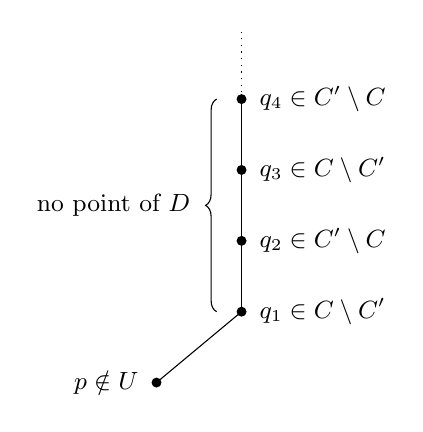
\begin{tikzpicture}[scale=0.9,every node/.style={font=\small}]
\foreach \i/\lab in {0/$q_1\in C\setminus C'$,1/$q_2\in C'\setminus C$,2/$q_3\in C\setminus C'$,3/$q_4\in C'\setminus C$}{
  \fill (0,\i) circle (2pt); \node[right=3pt] at (0,\i) {\lab};}
\draw (0,0)--(0,3); \draw[dotted] (0,3)--(0,4);
\fill (-1.2,-1) circle (2pt); \node[left=3pt] at (-1.2,-1) {$p\notin U$};
\draw (-1.2,-1)--(0,0);
\draw[decorate,decoration={brace,amplitude=4pt},xshift=-10pt] (0,0)--(0,3) node[midway,left=6pt] {no point of $D$};
\end{tikzpicture}
\hspace{2em}
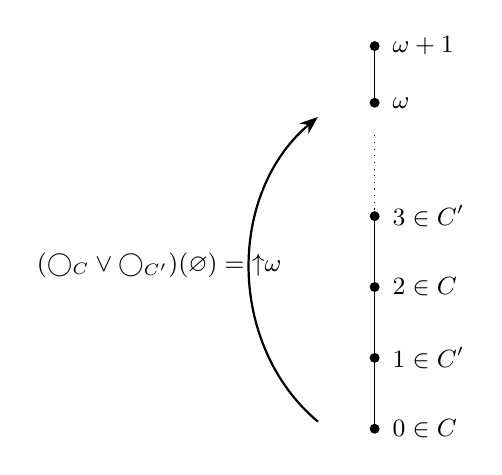
\begin{tikzpicture}[scale=0.9,every node/.style={font=\small}]
\foreach \i in {0,1,2,3} {\fill (0,\i) circle (2pt);}
\node[right=3pt] at (0,0) {$0\in C$}; \node[right=3pt] at (0,1) {$1\in C'$};
\node[right=3pt] at (0,2) {$2\in C$}; \node[right=3pt] at (0,3) {$3\in C'$};
\draw (0,0)--(0,3); \draw[dotted] (0,3)--(0,4.2);
\fill (0,4.6) circle (2pt); \node[right=3pt] at (0,4.6) {$\omega$};
\fill (0,5.4) circle (2pt); \node[right=3pt] at (0,5.4) {$\omega+1$};
\draw (0,4.6)--(0,5.4);
\draw[->,>=Stealth,thick] (-0.8,0.1) to[bend left=50] (-0.8,4.4);
\node[left=2pt] at (-1.1,2.3) {$(\lax_C\vee\lax_{C'})(\varnothing)=\upa\omega$};
\end{tikzpicture}
\caption{Left: a $D$-free alternating chain above a point $p\notin U$, the
obstruction of Theorem~\ref{thm:main}. Right: the chain $\omega+2$ with $C$
the even and $C'$ the odd finite ordinals; the alternating chain
$0<1<2<\cdots$ is $\varnothing$-free, and the join of the two nuclei sends
$\varnothing$ to $\upa\omega$, whereas $\lax_{C\cap C'}=\lax_\varnothing$ is
the constant $P$.}
\label{fig:chain}
\end{figure}

\begin{thm}[countable families]\label{thm:family}
Let $(C_i)_{i\in I}$ be a nonempty countable family of subsets of $P$ and $D=\bigcap_iC_i$. Then
$\bigvee_i\lax_{C_i}=\lax_D$ if and only if there is no infinite chain
$q_1<q_2<\cdots$ in $P\setminus D$ such that no point of $D$ lies in any
interval $[q_1,q_k]$ and every $C_i$ contains $q_k$ for infinitely many $k$.
\end{thm}
\begin{proof}
As before, $\bigvee_i\lax_{C_i}=\lax_D$ iff $\bigcap_i\Fix(\lax_{C_i})\subseteq
\Fix(\lax_D)$. Let $U$ be a common fixed point and $p\notin U$ a point with no
point of $D\setminus U$ above it. Choose a sequence of indices $i_1,i_2,\dots$
in which every index of $I$ occurs infinitely often. Put $q_0=p$ and, given
$q_{k-1}\notin U$, use $U\in\Fix(\lax_{C_{i_k}})$ to choose
$q_k\in C_{i_k}\setminus U$ with $q_k\ge q_{k-1}$; by assumption $q_k\notin D$.
The sequence is non-decreasing and is not eventually constant: a value $q$
taken for all large $k$ would lie in $C_i$ for every $i$, since every index
recurs, i.e.\ in $D$. Being non-decreasing and not eventually constant, it
takes each value only finitely many times. Its distinct values therefore form
an infinite chain in $P\setminus U$ in which each $C_i$ occurs infinitely
often, because $C_i$ contains $q_k$ for the infinitely many $k$ with $i_k=i$,
and which is $D$-free, because a point of $D$ below some value is
outside the up-set $U$ and above $p$. This contradicts the hypothesis, so
$U\in\Fix(\lax_D)$. Conversely, given a chain as in the statement, the up-set
$U=P\setminus\dn\{q_k\}$ is fixed by every $\lax_{C_i}$, since each $C_i$ is
cofinal in the chain, and $q_1\notin U$ lies below no point of $D\setminus U$;
so $U$ is a common fixed point not fixed by $\lax_D$, by the same computation.
\end{proof}

\begin{cor}\label{cor:embed}
Suppose every nonempty subset of $P$ has a maximal element (equivalently,
assuming dependent choice, $P$ has no infinite ascending chain). Then
$\bigvee_{i\in I}\lax_{C_i}=\lax_{\bigcap_iC_i}$ for every family
$(C_i)_{i\in I}$ of subsets of $P$, so that $C\mapsto\lax_C$ turns arbitrary
unions into meets and arbitrary intersections into joins; by Lindenhovius's
theorem it is then an isomorphism of complete lattices
$(\pow(P),\supseteq)\cong\Nuc(\Up(P))$. For every poset with an infinite
ascending chain there are $C,C'\subseteq P$ with
$\lax_C\vee\lax_{C'}\ne\lax_{C\cap C'}$.
\end{cor}
\begin{proof}
Let $D=\bigcap_iC_i$ (with $D=P$ and $\lax_D$ the identity if $I$ is empty),
let $U$ be fixed by every $\lax_{C_i}$ and let $p\notin U$. The set
$\upa p\setminus U$ is nonempty, so it has a maximal element $m$. For each
$i$, since $U\in\Fix(\lax_{C_i})$ there is $c_i\in C_i\setminus U$ with
$m\le c_i$, and maximality gives $c_i=m$; hence $m\in D\setminus U$ lies
above $p$. So $U\in\Fix(\lax_D)$, and $\bigcap_i\Fix(\lax_{C_i})\subseteq
\Fix(\lax_D)$ gives the equality of nuclei. Preservation of unions is
Lemma~\ref{lem:basic}(ii), and injectivity makes $C\mapsto\lax_C$ an
order-embedding of complete lattices; it is onto $\Nuc(\Up(P))$ by
\cite[Thm.~2.12]{Lindenhovius} applied to the dual poset, since every
nonempty subset of $P$ has a maximal element iff every nonempty subset of the
dual has a minimal element. For the last statement let $q_1<q_2<\cdots$ be an
infinite chain and put $C=\{q_i:i\text{ odd}\}$, $C'=\{q_i:i\text{ even}\}$;
then $D=\varnothing$ and the chain is $D$-free, so Theorem~\ref{thm:main}
applies.
\end{proof}

\begin{ex}\label{ex:examples}
(a) On $\omega+2$ with $C$ the even and $C'$ the odd finite ordinals, the
join sends $\varnothing$ to $\upa\omega$ and $\lax_\varnothing$ is constant;
this is the pair of nuclei used in \cite[\S5]{Laxjoin} to show that the join
is not expressible in the bimodal language.
(b) On $\omega+1$ with $C=\{\text{even}\}\cup\{\omega\}$ and
$C'=\{\text{odd}\}\cup\{\omega\}$, $D=\{\omega\}$ is above every finite
ordinal but inside no interval $[q_1,q_i]$ of the chain $0<1<2<\cdots$, so
the join differs from $\lax_D$: the up-set $\{\omega\}$ is fixed by $\lax_C$
and $\lax_{C'}$ but $\lax_D\{\omega\}=P$.
(c) On $\mathbb N$ with $C=\{n:n\equiv0,2,3\pmod4\}$ and
$C'=\{n:n\equiv0,1,3\pmod 4\}$ we have $C\setminus C'=\{n\equiv2\}$,
$C'\setminus C=\{n\equiv1\}$, and every interval $[q_1,q_2]$ with
$q_1\equiv2$, $q_2\equiv1$, $q_1<q_2$ contains $q_1+1\equiv3\in D$. Hence no
$D$-free alternating chain exists although $\mathbb N$ has infinite chains,
and $\lax_C\vee\lax_{C'}=\lax_D$.
\end{ex}

\begin{rem}
The pattern is that of the lattice of Grothendieck topologies inside the
lattice of classes of local isomorphisms \cite{Topjoin,Finitejoin}: there,
meets of topologies always go to joins of classes, and joins of topologies go
to meets of classes on finite categories but not on the poset $\mathbb N$.
Here, $C\mapsto\lax_C$ always turns unions into meets, and turns
intersections into joins exactly when the alternating chains of
Theorem~\ref{thm:main} are absent, which is automatic without infinite
ascending chains.
\end{rem}

\section{The induction scheme as a frame condition}\label{sec:frames}

A \emph{frame} is a triple $(P,C,C')$ with $P$ a poset and $C,C'\subseteq P$.
A valuation assigns up-sets to propositional variables; $\wedge,\vee,\to,\bot$
are interpreted in $\Up(P)$, $\laxa$ by $\lax_C$ and $\laxb$ by $\lax_{C'}$.
For the third connective $\lax$ there are two readings: the
\emph{intersection reading} $\lax=\lax_{C\cap C'}$ and the \emph{join
reading} $\lax=\lax_C\vee\lax_{C'}$, given by Proposition~\ref{prop:gfp}. The
two coincide on finite frames \cite[Thm.~4.1]{Laxjoin}.

\begin{thm}\label{thm:corr}
\begin{enumerate}
\item[(i)] Under the join reading every frame validates $\LLJ$.
\item[(ii)] Under the intersection reading a frame validates the inclusion
axioms $\laxa\varphi\to\lax\varphi$ and $\laxb\varphi\to\lax\varphi$ and the
lax axioms for $\lax$, and it validates the induction scheme (JL) if and only
if it has no $D$-free alternating chain, $D=C\cap C'$; in that case it
validates $\LLJ$.
\end{enumerate}
\end{thm}
\begin{proof}
(i) $\Up(P)$ is a complete Heyting algebra and $\lax_C,\lax_{C'}$ are nuclei,
so $(\Up(P),\lax_C,\lax_{C'},\lax_C\vee\lax_{C'})$ is an $\LLJ$-algebra by
\cite[Prop.~3.2]{Laxjoin}. (ii) $\lax_{C\cap C'}$ is a nucleus above
$\lax_C$ and $\lax_{C'}$, which gives the inclusion and lax axioms. If there
is no $D$-free alternating chain, $\lax_{C\cap C'}$ is the join by
Theorem~\ref{thm:main} and (i) applies. If there is one, then by
Theorem~\ref{thm:main} some up-set $U$ is fixed by $\lax_C$ and $\lax_{C'}$
but not by $\lax_D$; take a variable $p$ with value $U$ and the instance of
(JL) with $\psi=\varphi=p$. Its antecedents $\laxa p\to p$, $\laxb p\to p$ and
$p\to p$ have value $P$, while $\lax p\to p$ has value
$\lax_DU\to U\ne P$ because $\lax_DU\not\subseteq U$. So this instance of
(JL) fails.
\end{proof}

\begin{prop}\label{prop:nonfo}
The class of frames $(P,C,C')$ without $D$-free alternating chains is not
definable by any set of first-order sentences in the language of a binary
relation and two unary predicates. Hence the induction scheme (JL), under the
intersection reading, is not first-order definable as a frame condition.
\end{prop}
\begin{proof}
Suppose a set $\Sigma$ of sentences defined the class. Add constants
$c_1,c_2,\dots$ and the sentences $c_i<c_{i+1}$, $c_i\in C\setminus C'$ for
odd $i$, $c_i\in C'\setminus C$ for even $i$, and
$\neg\exists d\,(d\in C\wedge d\in C'\wedge c_1\le d\le c_i)$ for all $i$.
Every finite subset of $\Sigma$ together with these sentences has a model: a
finite chain $c_1<\cdots<c_n$ with the stated memberships is a finite frame,
which has no infinite chain at all and therefore satisfies $\Sigma$. By
compactness the whole set has a model, a frame in $\Sigma$'s class with a
$D$-free alternating chain, a contradiction.
\end{proof}

\begin{rem}
The analogy with common knowledge \cite{HM} is exact on this point: the
common-knowledge operator is the greatest fixed point $\nu X.\,E(\varphi\wedge
X)$, its induction axiom is valid on a frame exactly when the common-knowledge
relation is the transitive closure of the union of the agents' relations, and
that class is not first-order definable. Here $\lax_C\vee\lax_{C'}$ is the
greatest fixed point of Proposition~\ref{prop:gfp}, the induction scheme (JL)
is valid under the intersection reading exactly when the alternating chains
are absent, and this class is not first-order definable.
\end{rem}

\section{Every nucleus is a join of relativized necessities}\label{sec:dense}

On a poset with an infinite ascending chain some nuclei on $\Up(P)$ are not
relativized necessities \cite[Thm.~2.12]{Lindenhovius}; the join of the two
nuclei of Example~\ref{ex:examples}(a) is one. They are, however, joins of
relativized necessities, and the generators can be written down.

For $a\in H$ the \emph{closed} and \emph{open} nuclei are $c_a(b)=a\vee b$
and $u_a(b)=a\to b$; they generate $\Nuc(H)$ as a frame, and every nucleus
is the join of the nuclei $u_a\wedge c_{ja}$, $a\in H$ \cite[Ch.~II, \S2]{Johnstone}.
On $\Up(P)$ these generators are relativized necessities: for up-sets $U,V$,
\[
\lax_{U\cup(P\setminus V)}=u_U\wedge c_V,
\]
since $\upa x\cap(U\cup(P\setminus V))\subseteq W$ iff $\upa x\cap U\subseteq W$
and $\upa x\subseteq V\cup W$, i.e.\ $x\in(U\to W)\cap(V\cup W)$. In
particular $u_U=\lax_U$ and $c_V=\lax_{P\setminus V}$. The following
theorem is therefore the classical presentation in Alexandrov form, with a
direct proof.

\begin{thm}\label{thm:dense}
Let $P$ be a poset and $j$ a nucleus on $\Up(P)$. For $U\in\Up(P)$ and
$x\in jU\setminus U$ put $C(U,x)=P\setminus(\upa x\setminus U)=U\cup(P\setminus\upa x)$,
so that $\lax_{C(U,x)}=u_U\wedge c_{\upa x}$. Then
$\lax_{C(U,x)}\le j$, $U\notin\Fix(\lax_{C(U,x)})$, and
\[
j=\bigvee\{\lax_{C(U,x)}:\ U\in\Up(P),\ x\in jU\setminus U\}
=\bigvee\{\lax_C:\ C\subseteq P,\ \lax_C\le j\}.
\]
Hence the relativized necessities are join-dense in $\Nuc(\Up(P))$, and the
sublattice they generate consists of the finite joins
$\lax_{C_1}\vee\dots\vee\lax_{C_n}$, each given by the greatest fixed point of
Proposition~\ref{prop:gfp} with $n$ conditions.
\end{thm}
\begin{proof}
Write $C=C(U,x)$. Since $\upa x\cap C\subseteq U$ we have $x\in\lax_CU\setminus U$,
so $U$ is not fixed by $\lax_C$. For $\lax_C\le j$ we show
$\Fix(j)\subseteq\Fix(\lax_C)$. Let $V\in\Fix(j)$ and $z\notin V$, and suppose
that no point of $C$ above $z$ lies outside $V$, i.e.\
$\upa z\setminus V\subseteq\upa x\setminus U$. Then $z$ itself lies in
$\upa x\setminus U$, so $z\ge x$ and therefore $z\in jU$; and
$\upa z\cap U\subseteq V$, i.e.\ $z\in U\to V$, where $U\to V=\{w:\upa w\cap U
\subseteq V\}$ is the Heyting implication of $\Up(P)$. As $V$ is fixed by
$j$, so is $U\to V$: since $j$ preserves binary meets, $j(a\to b)\wedge ja
=j((a\to b)\wedge a)\le jb$ gives $j(a\to b)\le ja\to jb$, whence
$j(U\to V)\le jU\to jV=jU\to V\le U\to V$. Hence
$z\in jU\cap j(U\to V)=j(U\cap(U\to V))\subseteq jV=V$, a contradiction. So
every $z\notin V$ has a point of $C\setminus V$ above it, $V\in\Fix(\lax_C)$,
and $\lax_C\le j$.

Consequently $\Fix(j)\subseteq\Fix(\lax_{C(U,x)})$ for all $(U,x)$, with
$U\notin\Fix(\lax_{C(U,x)})$ for every $U\notin\Fix(j)$; so
$\Fix(j)=\bigcap_{(U,x)}\Fix(\lax_{C(U,x)})$, which is the first equality, and
the second follows since every $\lax_C\le j$ lies between $\lax_{C(U,x)}$'s
join and $j$. For the sublattice, meets of relativized necessities are
relativized necessities (Lemma~\ref{lem:basic}(ii)), and since $\Nuc(H)$ is a
frame \cite{Johnstone}, binary meets distribute over joins:
$(\lax_{C_1}\vee\dots\vee\lax_{C_n})\wedge\lax_E=\lax_{C_1\cup E}\vee\dots\vee
\lax_{C_n\cup E}$. The greatest-fixed-point description of an $n$-fold join is
proved as Proposition~\ref{prop:gfp}, with $X\subseteq\dn(X\cap C_i)$ required
for every $i$.
\end{proof}

\begin{rem}
The generators $\lax_{C(U,x)}=u_U\wedge c_{\upa x}$ refine the classical
generators $u_U\wedge c_{jU}$: as $jU=\bigcup_{x\in jU}\upa x$ and closed
nuclei turn joins into joins, $u_U\wedge c_{jU}=\bigvee_{x\in jU}(u_U\wedge
c_{\upa x})$ by frame distributivity, and the terms with $x\in U$ are below
the identity nucleus. What is specific to $\Up(P)$ is that these generators,
and hence all finite meets of open and closed nuclei, are induced by subsets
of $P$.
\end{rem}

\begin{ex}\label{ex:tree}
Finite joins do not suffice. For any poset, $\lax_C\le\neg\neg$ if and only
if $C$ is cofinal, i.e.\ every point has a point of $C$ above it: if
$\lax_C\le\neg\neg$ then $\lax_C\varnothing\subseteq\neg\neg\varnothing=
\varnothing$, so no point has $\upa x\cap C=\varnothing$; conversely, if $C$ is cofinal and $x\in\lax_CU$, then every $y\ge x$ has
a point $z\ge y$ in $C$, which lies in $U$, so $\upa y\cap U\ne\varnothing$
for all $y\ge x$, i.e.\ $x\in\neg\neg U$. Let
$T$ be the full binary tree, ordered by extension of finite $0$--$1$ words.
Given cofinal $C_1,\dots,C_n$, choose $x_1<x_2<\cdots$ with $x_k\in C_i$ for
$k\equiv i\pmod n$; then $B=\dn\{x_k\}$ is an infinite branch and $U=T\setminus
B$ is an up-set fixed by every $\lax_{C_i}$, each $C_i$ being cofinal in $B$.
But $\neg U=\{t:\upa t\cap U=\varnothing\}$ is empty: a node $t\notin B$
lies in $U$, and a node $t\in B$ has two children, of which the one not on
$B$ lies in $U$; so every node has a descendant in $U$, and
$\neg\neg U=T\ne U$. Hence $\neg\neg$ on $\Up(T)$ is not a join of finitely
many relativized necessities, while by Theorem~\ref{thm:dense} it is the join
of all $\lax_C$ with $C$ cofinal. \end{ex}

\begin{prop}\label{prop:omega}
Every nucleus on $\Up(\omega)$ is a join of at most two relativized
necessities; for instance $\neg\neg=\lax_{\mathrm{even}}\vee\lax_{\mathrm{odd}}$.
\end{prop}
\begin{proof}
The up-sets of $\omega$ are $\varnothing$ and the tails $\upa n$, and
$\Fix(\lax_C)$ consists of $\omega$, the tails $\upa(c+1)$ for $c\in C$, and
$\varnothing$ exactly when $C$ is infinite. The fixed-point set $S$ of a
nucleus contains $\omega$ and is closed under intersections, so if it
contains infinitely many tails it contains $\varnothing$. Let $A=\{c:\upa(c+1)
\in S\}$. If $A$ is infinite, or if $A$ is finite and $\varnothing\notin S$,
then $S=\Fix(\lax_A)$. If $A$ is finite and $\varnothing\in S$, split
$\omega\setminus A$ into two disjoint infinite sets $E$ and $O$; then
$\Fix(\lax_{A\cup E})\cap\Fix(\lax_{A\cup O})=S$, so the nucleus is
$\lax_{A\cup E}\vee\lax_{A\cup O}$. For $\neg\neg$, $S=\{\varnothing,\omega\}$
and $A=\varnothing$.
\end{proof}

\begin{que}
Which nuclei on $\Up(P)$ are joins of finitely many relativized necessities?
On $\omega$ two always suffice (Proposition~\ref{prop:omega}); on the binary
tree $\neg\neg$ needs infinitely many (Example~\ref{ex:tree}).
\end{que}

\section*{Funding}
No funding was received for this work.

\section*{Declarations}
The author has no competing interests to declare.

\begin{thebibliography}{9}
\bibitem{Escardo} M.~H.~Escard\'o, \emph{Joins in the frame of nuclei}, Appl.
Categ. Structures \textbf{11} (2003), 117--124.
\bibitem{Goldblatt} R.~Goldblatt, \emph{Grothendieck topology as geometric
modality}, Z. Math. Logik Grundlag. Math. \textbf{27} (1981), 495--529.
\bibitem{Hemelaer} J.~Hemelaer, \emph{Grothendieck topologies on posets},
preprint, arXiv:1811.10039, 2018.
\bibitem{HM} J.~Y.~Halpern, Y.~Moses, \emph{Knowledge and common knowledge in a
distributed environment}, J. ACM \textbf{37} (1990), 549--587.
\bibitem{Johnstone} P.~T.~Johnstone, \emph{Stone Spaces}, Cambridge University
Press, 1982.
\bibitem{Lindenhovius} B.~Lindenhovius, \emph{Grothendieck topologies on a
poset}, preprint, arXiv:1405.4408, 2014.
\bibitem{Macnab} D.~S.~Macnab, \emph{Modal operators on Heyting algebras},
Algebra Universalis \textbf{12} (1981), 5--29.
\bibitem{Laxjoin} R.~Shibusawa, \emph{The join of two nuclei as a lax modality:
axiomatization, finite models, and inexpressibility}, preprint, 2026,
DOI 10.5281/zenodo.23330576.
\bibitem{Topjoin} R.~Shibusawa, \emph{Meets and joins of Grothendieck
topologies in the sameness lattice}, preprint, 2026, DOI 10.5281/zenodo.22978446.
\bibitem{Finitejoin} R.~Shibusawa, \emph{Grothendieck topologies on a finite
category form a sublattice of the lattice of two-out-of-three classes},
preprint, 2026, DOI 10.5281/zenodo.23204943.
\end{thebibliography}

\end{document}
